\documentclass[t,usenames,dvipsnames]{beamer}
\usetheme{Copenhagen}
\setbeamertemplate{headline}{} % remove toc from headers
\beamertemplatenavigationsymbolsempty

\usepackage{amsmath, xcolor, tikz, pgfplots, array, cancel}

\pgfplotsset{compat = newest}
\usetikzlibrary{arrows.meta, calc, decorations.pathreplacing}
\pgfplotsset{every axis/.append style = {axis lines = middle}}
\pgfplotsset{every tick label/.append style={font=\scriptsize}}
\everymath{\displaystyle}

\title{Sequences}
\author{}
\date{}

\AtBeginSection[]
{
  \begin{frame}
    \frametitle{Objectives}
    \tableofcontents[currentsection]
  \end{frame}
}

\begin{document}

\begin{frame}
    \maketitle
\end{frame}

\section{List the terms of an explicit sequence.}

\begin{frame}{Sequences}
An \alert{sequence} $\{a_n\}$ is a list of numbers written as a function whose domain is the set of non-negative integers (\textit{i.e.} 0, 1, 2, $\dots$).  \newline\\  \pause

We will mostly stick with positive integers (1, 2, 3, $\dots$).   \newline\\  \pause

The function values (\textbf{terms}) are $a_1, a_2, a_3, a_4, \dots, a_n$; or $a_0, a_1, a_2, a_3, \dots, a_n$ if using a starting value of 0.
\end{frame}

\begin{frame}{Sequences}
The value $a(n)$ is often written as $a_n$ and is called the $n^\text{th}$ term of the sequence. \newline\\

The sequence is denoted by $a_n$ or $\{a_n\}^{\infty}_{n=1}$. \newline\\ \pause

We list out the terms of a sequence by substituting values of $n$ into the sequence's definition. \newline\\ \pause

\emph{Note:} We can use any variable to name a sequence $a_n, \, b_n, \, c_n,$ etc.  We can also use any letter we want instead of $n$.
\end{frame}

\begin{frame}{Example 1}
Write the first 4 terms of the sequence whose explicit rule is given.  \newline\\
(a) \quad $a_n = \dfrac{5^{n-1}}{3^n}$   
\begin{center}
\begin{align*}
    \onslide<2->{a(1) &= \frac{5^{1-1}}{3^1} = \frac{1}{3}&} \qquad
    \onslide<3->{a(2) = \frac{5^{2-1}}{3^2} = \frac{5}{9}&} \\[0.5cm]
    \onslide<4->{a(3) &= \frac{5^{3-1}}{3^3} = \frac{25}{27}&} \qquad
    \onslide<5->{a(4) = \frac{5^{4-1}}{3^4} = \frac{125}{81}&} \\
\end{align*}
\end{center}
\end{frame}

\begin{frame}{Example 1}
(b) \quad $b_k = \frac{(-1)^k}{2k+1}, \, k \geq 0$
\begin{center}
\begin{align*}
    \onslide<2->{b(0) &= \frac{(-1)^0}{2(0)+1} = 1&} \qquad
    \onslide<3->{b(1) = \frac{(-1)^1}{2(1)+1} = -\frac{1}{3}&} \\[0.5cm]
    \onslide<4->{b(2) &= \frac{(-1)^2}{2(2)+1} = \frac{1}{5}&} \qquad
    \onslide<5->{b(3) = \frac{(-1)^3}{2(3)+1} = -\frac{1}{7}&} \\
\end{align*}
\end{center}
\end{frame}

\begin{frame}{Example 1}
(c) \quad $\{2n-1\}_{n=1}^{\infty}$
\begin{center}
\begin{align*}
    \onslide<2->{c(1) &= 2(1)-1 = 1&} \qquad
    \onslide<3->{c(2) &= 2(2)-1 = 3&} \\[0.5cm]
    \onslide<4->{c(3) &= 2(3)-1 = 5&} \qquad
    \onslide<5->{c(4) &= 2(4)-1 = 7&} \\
\end{align*}
\end{center}
\end{frame}

\begin{frame}{Example 1}
(d) \quad $\left\{\frac{1+(-1)^i}{i}\right\}_{i=2}^{\infty}$
\begin{center}
\begin{align*}
    \onslide<2->{c(2) &= \frac{1+(-1)^2}{2} = 1&} \qquad
    \onslide<3->{c(3) &= \frac{1+(-1)^3}{3} = 0&} \\[0.5cm]
    \onslide<4->{c(4) &= \frac{1+(-1)^4}{4} = \frac{1}{2}&} \qquad
    \onslide<5->{c(5) &= \frac{1+(-1)^5}{5} = 0&} \\
\end{align*}
\end{center}
\end{frame}

\begin{frame}{Graphs of Sequences}
We can graph a sequence by using coordinates.  

\[ a_n = \frac{1}{n}    \]
\begin{center}
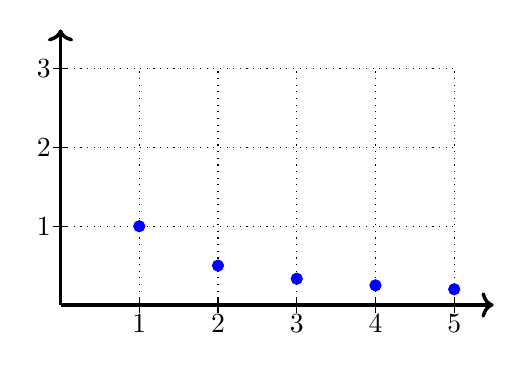
\begin{tikzpicture}
\draw [dotted] (0,0) grid (5,3);
\draw [->, line width = 1.25] (0,0) -- (5.5,0);
\draw [->, line width = 1.25] (0,0) -- (0,3.5);
\foreach \x in {1,2,...,5}
\draw (\x, -0.1) -- (\x, 0.1);
\foreach \x in {1,2,...,5}
\node at (\x, 0) [anchor = north] {$\x$};
\foreach \y in {1,2,3}
\draw (-0.1,\y) -- (0.1,\y);
\foreach \y in {1,2,3}
\node at (0,\y) [anchor = east] {$\y$};
\foreach \x in {1,2,...,5}
\draw [fill=blue, color=blue] (\x, 1/\x) circle (2pt);
\end{tikzpicture}
\end{center}
\end{frame}

\section{List the terms of a recursive sequence.}

\begin{frame}{Recursive Sequences}
A \alert{recursive sequence} is one that is defined using previous terms.  \newline\\   \pause

You are given a starting term value and then a rule for generating additional terms.  \newline\\    \pause

The notations for successive terms are either
\[  a_n \text{ and } a_{n+1} \]
or
\[  a_{n-1} \text{ and } a_n \]
\end{frame}

\begin{frame}{Example 2}
Write the first four terms of each sequence.    \newline\\
(a) \quad $a_1=5 \text{ and } a_n = 3a_{n-1}+2 \text{ for } n \geq 2$
\begin{center}
\onslide<2->{Each new term = (3 $\times$ previous term) + 2}
\begin{align*}
    \onslide<3->{a_1 &= 5&} \qquad
    \onslide<4->{a_2 &= 3(5)+2 = 17&} \\[0.5cm]
    \onslide<5->{a_3 &= 3(17)+2 = 53&} \qquad
    \onslide<6->{a_4 &= 3(53)+2 = 161&} 
\end{align*}
\end{center}
\end{frame}

\begin{frame}{Example 2}
(b) \quad $a_1=7 \text{ and } a_{n+1} = 2-a_n \text{ for } n \geq 1$
\begin{center}
\onslide<2->{Each new term = 2 -- previous term}
\begin{align*}
    \onslide<3->{a_1 &= 7&} \qquad
    \onslide<4->{a_2 &= 2-7 = -5&} \\[0.5cm]
    \onslide<5->{a_3 &= 2-(-5) = 7&} \qquad
    \onslide<6->{a_4 &= 2-7 = -5&} 
\end{align*}
\end{center}
\end{frame}

\begin{frame}{Example 2}
(c) \quad $f_0=1 \text{ and } f_n = n\cdot f_{n-1} \text{ for } n \geq 1$
\begin{center}
\onslide<2->{Each new term = (term number) $\times$ (previous term)}
\begin{align*}
    \onslide<3->{f_0 &= 1&} \qquad
    \onslide<4->{f_1 &= 1(1) = 1&} \\[0.5cm]
    \onslide<5->{f_2 &= 2(1) = 2&} \qquad
    \onslide<6->{f_3 &= 3(2) = 6&} 
\end{align*}
\end{center}
\end{frame}

\section{Understand factorial notation}

\begin{frame}{Factorial Notation}
Products of consecutive positive integers can be expressed using factorial notation.  \newline\\ \pause

If $n$ is a positive integer, then
\[
n! = n(n-1)(n-2)\cdots (3)(2)(1)
\]

By definition, $0!=1$.
\end{frame}

\begin{frame}{Factorial Values}
Factorial values grow very quickly.
\begin{align*}
    1! &= 1     \\
    2! &= 2\cdot 1 = 2  \\
    3! &= 3\cdot 2\cdot 1 = 6   \\
    4! &= 4\cdot 3\cdot 2\cdot 1 = 24   \\
    5! &= 5\cdot 4\cdot 3\cdot 2\cdot 1 = 120   \\
    6! &= 6\cdot 5\cdot 4\cdot 3\cdot 2\cdot 1 = 720 \\
\end{align*}
\end{frame}

\begin{frame}{Grouping Symbols}
  Unless grouping symbols, like () are involved, factorials only affect the number or variable they follow.    \newline\\

$2 \cdot 3! = 2(3\cdot 2\cdot 1) = 12$, but $(2\cdot 3)! = 6! = 720$.   \newline\\ 
\end{frame}

\begin{frame}{Example 3}
Write the first 4 terms of each sequence.   \newline\\
(a) \quad $a_n = \dfrac{2^n}{(n-1)!}$
\begin{center}
\begin{align*}
    \onslide<2->{a_1 &= \frac{2^1}{(1-1)!} = 2&} \qquad
    \onslide<3->{a_2 &= \frac{2^2}{(2-1)!} = 4&} \\[0.5cm]
    \onslide<4->{a_3 &= \frac{2^3}{(3-1)!} = 4&} \qquad
    \onslide<5->{a_4 &= \frac{2^4}{(4-1)!} = \frac{8}{3}&} 
\end{align*}
\end{center}
\end{frame}

\begin{frame}{Example 3}
Write the first 4 terms of each sequence.   \newline\\
(b) \quad $b_n = \dfrac{20}{(n+1)!}$
\begin{center}
\begin{align*}
    \onslide<2->{b_1 &= \frac{20}{(1+1)!} = 10&} \qquad
    \onslide<3->{b_2 &= \frac{20}{(2+1)!} = \frac{10}{3}&} \\[0.5cm]
    \onslide<4->{b_3 &= \frac{20}{(3+1)!} = \frac{5}{6}&} \qquad
    \onslide<5->{b_4 &= \frac{20}{(4+1)!} = \frac{1}{6}&} 
\end{align*}
\end{center}
\end{frame}

\begin{frame}{Simplifying Factorial Expressions}
When simplifying factorial expressions, it helps to remember that
\[n! = n(n-1)(n-2)\cdots(3)(2)(1)  \]
\end{frame}

\begin{frame}{Example 4}
Simplify each.  \newline\\
(a) \quad $\dfrac{(n+1)!}{n!}$
\begin{align*}
    \onslide<2->{\frac{(n+1)!}{n!} &= \frac{(n+1)(n)(n-1)(n-2)\cdots(2)(1)}{n(n-1)(n-2)\cdots(2)(1)}}    \\[10pt]
    \onslide<3->{&= \frac{(n+1)\cancel{(n)}\cancel{(n-1)}\cancel{(n-2)}\cancel{\cdots}\cancel{(2)}\cancel{(1)}}{\cancel{(n)}\cancel{(n-1)}\cancel{(n-2)}\cancel{\cdots}\cancel{(2)}\cancel{(1)}}}    \\[10pt]
    \onslide<4->{&= n+1}
\end{align*}
\end{frame}

\begin{frame}{Example 4}
Simplify each.  \newline\\
(b) \quad $\dfrac{n!}{(n-1)!}$
\begin{align*}
    \onslide<2->{\frac{n!}{(n-1)!} &= \frac{n(n-1)(n-2)\cdots(2)(1)}{(n-1)(n-2)\cdots(2)(1)}}    \\[10pt]
    \onslide<3->{&= \frac{n\cancel{(n-1)}\cancel{(n-2)}\cancel{\cdots}\cancel{(2)}\cancel{(1)}}{\cancel{(n-1)}\cancel{(n-2)}\cancel{\cdots}\cancel{(2)}\cancel{(1)}}}    \\[10pt]
    \onslide<4->{&= n}
\end{align*}
\end{frame}

\section{Find terms of an arithmetic sequence}

\begin{frame}{Arithmetic Sequences}
When the difference between consecutive terms of a sequence is always the same, such as 8, 11, 14, 17, $\dots$, that sequence is an \alert{arithmetic sequence}.   \newline\\ \pause

The difference between those consecutive terms is called the \alert{common difference}. \newline\\    \pause

To find the common difference of an arithmetic sequence, {\color{blue}\textbf{subtract}} any two consecutive terms.  
\end{frame}

\begin{frame}{Arithmetic Sequences and Linear Functions}
Arithmetic sequences model linear functions.    \newline\\  \pause

The following graph shows the first 4 terms of the sequence 8, 11, 14, 17:
\newline\\
\begin{center}
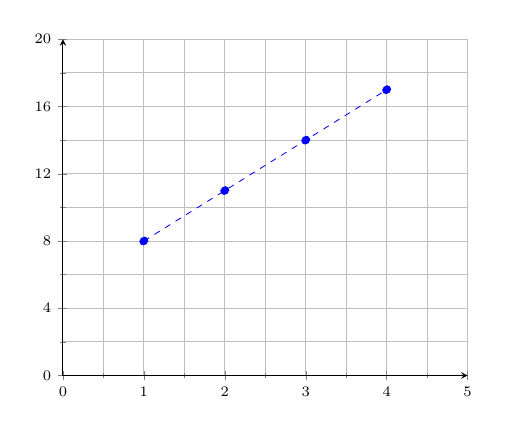
\begin{tikzpicture}[scale=0.75]
	\begin{axis}[
		axis lines = left,
		grid = both,
		xmin = 0, xmax = 5,
		ymin = 0, ymax = 20,
		ytick = {0,4,...,20},
		minor tick num = 1
	]
	\addplot [mark = *, color = blue, dashed] coordinates{
	(1, 8)
	(2, 11)
	(3, 14)
	(4, 17)
	};
	\end{axis}
\end{tikzpicture}
\end{center}
\end{frame}

\begin{frame}{Find the Rule for the Sequence}
Notice that the common difference between terms (3 in this case) is the same as the slope of the line.	\newline\\  \pause

If we subtract that 3 from the first term, we get 5; which is the $y$-intercept of the graph.	\newline\\  \pause

Thus, a sequence rule for this sequence is 
\[
y = 3x + 5 \qquad	\text{or}	\qquad	a_n = 3n+5 \text{ for } n \geq 1
\]
\end{frame}

\begin{frame}{Example 5}
Find an explicit formula for the $n^\text{th}$ term of each of the following sequences. \newline\\
(a) \quad $-31, \, -24, \, -17, \, -10, \dots$  \newline\\

\onslide<2->{Common Difference: $-24-(-31) = 7$}    \newline\\
\onslide<3->{$y$-intercept: $-31-7=-38$} \newline\\
\onslide<4->{\[a_n = 7n - 38\]}
\end{frame}

\begin{frame}{Example 5}
(b) \quad $37, \, 67, \, 97, \, 127, \dots$ \newline\\

\onslide<2->{Common Difference: $67-37=30$}    \newline\\
\onslide<3->{$y$-intercept: $37-30=7$} \newline\\
\onslide<4->{\[b_n = 30n + 7\]}
\end{frame}

\section{Find terms of a geometric sequence}

\begin{frame}{Geometric Sequences}
A \alert{geometric sequence} is one in which each term after the first is obtained by multiplying the preceding term by a fixed nonzero constant $r$ (called the {\color{blue}\textbf{common ratio}}). \newline\\  \pause

Geometric sequences model exponential growth or decay.  \newline\\
\end{frame}

\begin{frame}{Model of a Geometric Sequence}
The following graph shows the first 4 terms of the sequence 3, 6, 12, 24:  \newline\\
\begin{center}
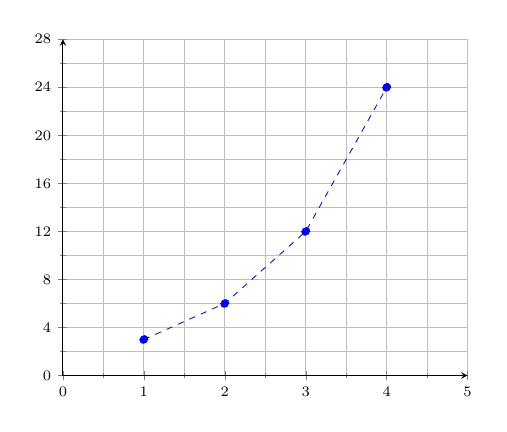
\begin{tikzpicture}[scale=0.75]
\begin{axis}[
axis lines = left,
grid = both,
xmin = 0, xmax = 5,
ymin = 0, ymax = 28,
ytick = {0,4,...,28},
minor tick num = 1
]
\addplot [mark = *, color = blue, dashed] coordinates{
	(1, 3)
	(2, 6)
	(3, 12)
	(4, 24)
};
\end{axis}
\end{tikzpicture}
\end{center}
\end{frame}

\begin{frame}{Finding Rule for Geometric Sequences}
Notice each point's $y$-coordinate is twice the previous one. This indicates that the common ratio, $r$, is the base of the exponential function, or 2.	\newline\\  \pause

To find the $y$-intercept, divide the first term by the base of 2 to get 1.5.	\newline\\  \pause

Thus, the function can be modeled as 
\[
y = 1.5\left(2\right)^x	\qquad \text{or} \qquad a_n = 1.5\left(2\right)^n \text{ for } n \geq 1
\]
\pause

**\emph{Note:} Unlike exponential functions, geometric sequences can have negative common ratios.
\end{frame}

\begin{frame}{Example 6}
Find the 8th term of each geometric sequence.   \newline\\  
(a) \quad $a_1=-4 \quad r=-2$   \newline\\
\onslide<2->{$y$-intercept: $2$} 
\begin{align*}
\onslide<3->{a_n &= 2\left(-2\right)^n} \\[6pt]
\onslide<4->{a_8 &= 2\left(-2\right)^8} \\[6pt]
\onslide<5->{a_8 &= 512}
\end{align*}
\end{frame}

\begin{frame}{Example 6}
Find the 8th term of each geometric sequence.   \newline\\  
(b) \quad $a_1=80 \quad r = 0.5$   \newline\\
\onslide<2->{$y$-intercept: $160$} 
\begin{align*}
\onslide<3->{a_n &= 160\left(0.5\right)^n} \\[6pt]
\onslide<4->{a_8 &= 160\left(0.5\right)^8} \\[6pt]
\onslide<5->{a_8 &= \frac{5}{8}}
\end{align*}
\end{frame}

\begin{frame}{Example 6}
(c) \quad $a_3 = -48 \quad a_5 = -768$  \newline\\
\begin{center}
\onslide<2->{
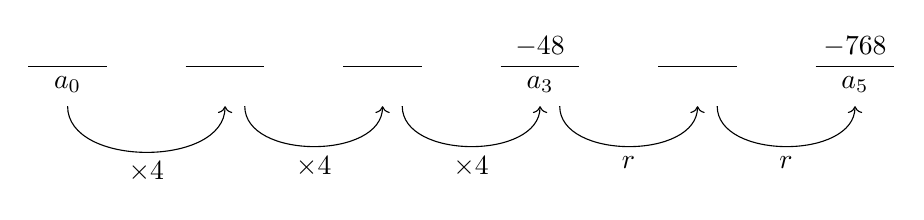
\begin{tikzpicture}
\draw (0,0) -- (1,0);
\draw (2,0) -- (3,0);
\draw (4,0) -- (5,0);
\draw (6,0) -- (7,0) node [midway, above] {$-48$};
\draw (8,0) -- (9,0);
\draw (10,0) -- (11,0) node [midway, above] {$-768$};
\node at (6.5,0) [below] {$a_3$};
\node at (10.5,0) [below] {$a_5$};
\onslide<3->{\draw [->] (6.75,-0.5) to [out=270, in=270] node [below, midway] {$r$} (8.5,-0.5);
\draw [->] (8.75,-0.5) to [out=270, in=270] node [below, midway] {$r$} (10.5,-0.5);
}
\onslide<8->{
\draw [->] (0.5,-0.5) to [out=270, in=270] node [below, midway] {$\times 4$} (2.5,-0.5);
\draw [->] (2.75,-0.5) to [out=270, in=270] node [below, midway] {$\times 4$} (4.5,-0.5);
\draw [->] (4.75,-0.5) to [out=270, in=270] node [below, midway] {$\times 4$} (6.5,-0.5);
}
\onslide<7->{\node at (0.5,0) [below] {$a_0$};}
\end{tikzpicture}}
\end{center}
\begin{align*}
    \onslide<4->{-48r^2 &= -768} \\
    \onslide<5->{r^2 &= 16} \\
    \onslide<6->{r &= \pm 4}
\end{align*}
\end{frame}

\begin{frame}{Example 6 \quad $a_3 = -48 \quad a_5 = -768$}
    \begin{align*}
        64a_0 &= -48 \\[6pt]
        \onslide<2->{a_0 &= -0.75}  \\[8pt]
        \onslide<3->{a_n &= -0.75(4)^n} \\[8pt]
        \onslide<4->{a_8 &= -0.75(4)^8} \\[8pt]
        \onslide<5->{&= -49,152}
    \end{align*}
\end{frame}

\begin{frame}{Example 6}
(d) \quad $a_1 = 5 \quad a_4 = 16.875$
\begin{align*}
    \onslide<2->{5r^3 &= 16.875} \\[8pt]
    \onslide<3->{r^3 &= 3.375} \\[8pt]
    \onslide<4->{r &= 1.5}  \\[8pt]
    \onslide<5->{a_0 &= 5/1.5} \\[8pt]
    \onslide<6->{a_0 &= \frac{10}{3}}
\end{align*}
\end{frame}

\begin{frame}{Example 6}
\begin{align*}
    a_n &= \frac{10}{3}\left(1.5\right)^n \\[12pt]
    \onslide<2->{a_8 &= \frac{10}{3}\left(1.5\right)^8} \\[12pt]
    \onslide<3->{&= \frac{10,935}{128}}
\end{align*}
\end{frame}

\begin{frame}{Example 7}
Write an explicit rule for each geometric sequence. \newline\\
(a) \quad 3, 6, 12, 24, 48, \dots   \newline\\
\onslide<2->{Common ratio = 6/3 = 2}    \newline\\
\onslide<3->{$y$-intercept = 1.5}
\onslide<4->{\[a_n = 1.5(2)^n\]}
\end{frame}

\begin{frame}{Example 7}
(b) \quad $2, \, -10, \, 50, \, -250,\, 1250, \, \dots$   \newline\\
\onslide<2->{Common ratio = $-10/2 = -5$}    \newline\\
\onslide<3->{$y$-intercept = $-\tfrac{2}{5}$}
\onslide<4->{\[b_n = -\frac{2}{5}\left(-5\right)^n\]}
\end{frame}
\end{document}

\begin{frame}{Example 7}
(c) \quad 5, 15, 45, 135, \dots   \newline\\
\onslide<2->{Common ratio = 15/5 = 3}    \newline\\
\onslide<3->{$y$-intercept = $\tfrac{5}{3}$}
\onslide<4->{\[c_n = \frac{5}{3}\left(3\right)^n\]}
\end{frame}

\end{document}
